\documentclass[conference]{IEEEtran}
\IEEEoverridecommandlockouts
% The preceding line is only needed to identify funding in the first footnote. If that is unneeded, please comment it out.
\usepackage{cite}
\usepackage{amsmath,amssymb,amsfonts}
\usepackage{algorithmic}
\usepackage{graphicx}
\usepackage{textcomp}
\usepackage{booktabs}
\usepackage{xcolor}
\def\BibTeX{{\rm B\kern-.05em{\sc i\kern-.025em b}\kern-.08em
    T\kern-.1667em\lower.7ex\hbox{E}\kern-.125emX}}
\begin{document}

\title{A Near Real-Time ISAC and Localization Platform using srsRAN\\}

\author{\IEEEauthorblockN{Samanvitha Balijepalli}
\IEEEauthorblockA{\textit{Dept. of ECE} \\
\textit{Rice University}\\
Houston, USA \\
sb273@rice.edu}
\and
\IEEEauthorblockN{Aniket Jadhav}
\IEEEauthorblockA{\textit{Dept. of ECE} \\
\textit{Rice University}\\
Houston, USA \\
aj156@rice.edu}
\and
\IEEEauthorblockN{Sandra Mansour}
\IEEEauthorblockA{\textit{Dept. of ECE} \\
\textit{Rice University}\\
Houston, USA  \\
sm367@rice.edu}
\and
}

\maketitle

\begin{abstract}
Detecting malicious or unauthorized signals such as jammers typically requires specialized sensing hardware, which is expensive to deploy, maintain, and upgrade. These systems are also difficult to adapt when detection requirements change or new signal types emerge. Most existing jammer detection and localization methods rely on continuous channel monitoring and time-domain techniques such as energy detection and correlation, which can limit flexibility and increase overhead. This project proposes a software-based approach using srsRAN as a flexible 5G platform for jammer detection and localization without requiring hardware modification. First, the project investigates how sensing opportunities can be introduced within the 5G protocol using Sounding Reference Signals (SRS). Second, it explores localization of jamming sources by extracting frequency-domain features from these standard reference signals through periodic sensing. Traditional indoor time-domain methods report 90th-percentile localization errors of 20–25 m; our target is 1–3 m accuracy using existing srsRAN-compatible hardware.
\end{abstract}

\begin{IEEEkeywords}
Integrated Sensing and Communication (ISAC), Jammer detection, jammer localization, srsRAN, 5G NR, Sounding Reference Signals (SRS), wireless sensing, channel estimation, frequency-domain feature extraction

\end{IEEEkeywords}

\section{Introduction}
The evolution of wireless communication toward sixth-generation (6G) networks has introduced the paradigm of Integrated Sensing and Communication (ISAC), where communication infrastructure can simultaneously support environmental sensing and localization tasks. By utilizing existing wireless signals for both data transmission and sensing, ISAC architectures enable efficient spectrum utilization while supporting applications such as indoor localization, environmental mapping, and context-aware networking. However, many existing sensing implementations rely on specialized radar hardware or proprietary platforms, limiting their accessibility and flexibility for experimental research. This motivates the development of open and programmable sensing platforms based on software-defined radio (SDR) frameworks and open radio access network (O-RAN) architectures.

A variety of signal processing algorithms have been proposed for estimating spatial parameters such as direction-of-arrival (DoA) and propagation delay from wireless measurements. Classical subspace-based techniques such as MUSIC \cite{1143830}, Root-MUSIC \cite{45540}, and ESPRIT \cite{32276} provide high-resolution parameter estimation by exploiting the structure of signal and noise subspaces, while adaptive beamforming methods such as Minimum Variance Distortionless Response (MVDR) \cite{articles} improve spatial selectivity and interference suppression. More recent approaches, including sparse direction-of-arrival estimation \cite{inbook}, leverage sparsity in the spatial domain to enhance estimation performance in multipath environments. In addition, systems such as SpotFi \cite{article} have demonstrated that joint angle-of-arrival and time-of-flight estimation from channel state information can enable decimeter-level localization using commodity wireless hardware.

In this work, we develop a sensing platform that integrates high-resolution parameter estimation algorithms within an open radio access network framework. The proposed system leverages the srsRAN \cite{srsran_docs} software stack deployed in an O-RAN compatible cloud environment to enable flexible signal acquisition, processing, and experimentation. Within this architecture, benchmark sensing algorithms including MUSIC \cite{1143830}, Root-MUSIC \cite{45540}, ESPRIT \cite{32276}, MVDR \cite{articles} beamforming, sparse DoA estimation \cite{inbook}, and \cite{article} SpotFi-inspired joint angle-delay estimation are implemented and systematically evaluated. This platform provides a unified experimental testbed for studying sensing performance, multipath resolution, and localization accuracy, while enabling practical exploration of ISAC concepts using open-source communication infrastructure.

\begin{figure}[htbp]
    \centering
    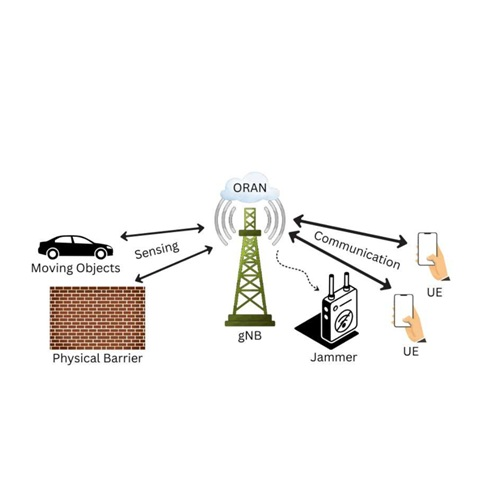
\includegraphics[width=0.8\linewidth, trim={1cm 1cm 1cm 3.5cm}, clip]{figures/Capstone Image.jpeg}
    \caption{Joint communication and sensing framework for jammer detection}
    \label{fig:Capstone_Image}
\end{figure}



\section{Methodology}
\subsection{System Architecture}

The proposed system is built on the srsRAN 5G software stack deployed within an Open Radio Access Network (O-RAN) compatible cloud environment, providing a flexible infrastructure for wireless signal acquisition and processing. Within the communication stack, physical-layer operations such as synchronization, OFDM demodulation, and channel estimation are performed to extract structured channel measurements from received signals. These measurements serve as the input for higher-level sensing analysis.

The sensing subsystem operates as an additional processing layer that analyzes channel measurements derived from the communication pipeline in order to estimate spatial and temporal propagation parameters. These parameters enable characterization of multipath components and support applications such as localization and environmental awareness. By embedding sensing modules within the communication processing chain, the architecture allows multiple signal processing techniques to be evaluated under identical signal conditions. This modular design provides a unified experimental platform for studying wireless sensing performance and exploring integrated sensing and communication capabilities within open-source radio access networks.

\begin{figure}[htbp]
    \centering
    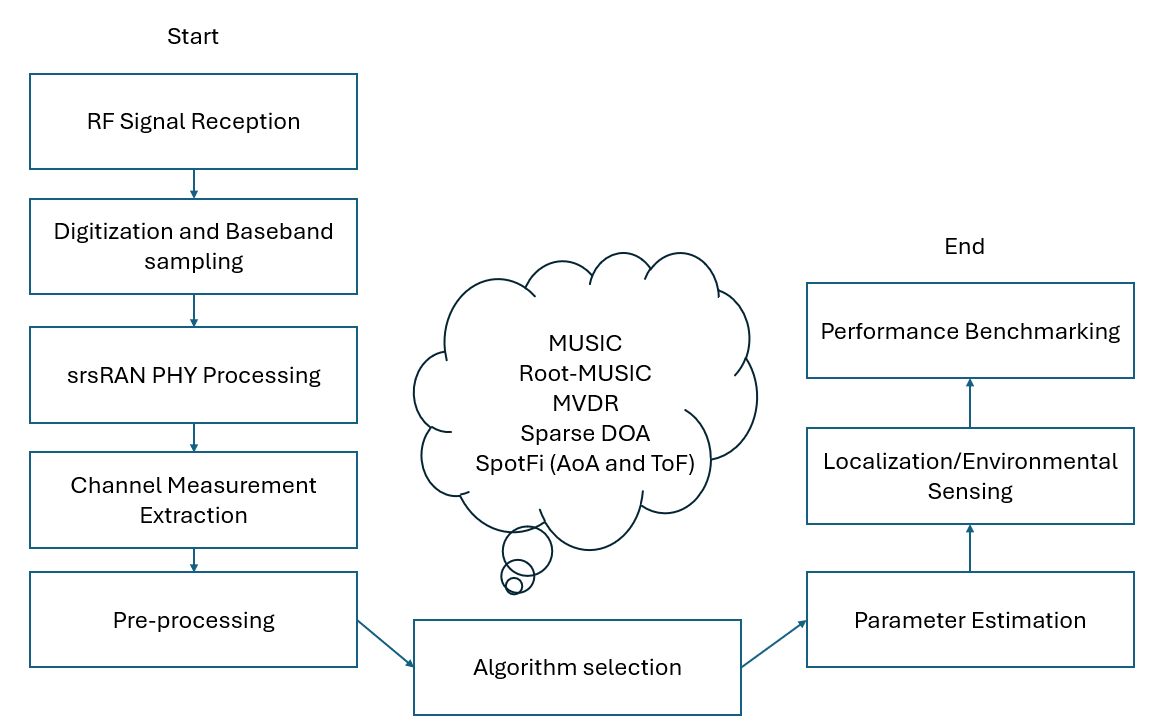
\includegraphics[width=0.8\linewidth]{figures/Screenshot 2026-03-13 215206.png}
    \caption{System architecture and processing flow for the proposed sensing framework.}
    \label{fig:system_flowchart}
\end{figure}

\subsection{SRS Configuration Space Analysis}

To determine feasible sensing configurations, relevant 3GPP NR specifications were reviewed to identify the protocol-defined design space for Sounding Reference Signals (SRS) across the PHY, RRC, DCI, MAC, and uplink power-control layers. This analysis identified key sensing-related parameters including SRS antenna ports $\{1,2,4\}$, symbol counts $\{1,2,4\}$, comb sizes $\{2,4\}$, and periodicities 
$T_{SRS} \in \{1,2,4,5,8,10,16,20,32,40,64,80,160,320,640,1280,2560\}$ slots.

Additional Radio Resource Control (RRC) parameters relevant to SRS resource design were documented, including $startPosition = 0$--$5$, $repetitionFactor \in \{1,2,4\}$, $freqDomainPosition = 0$--$67$, and $freqDomainShift = 0$--$268$. Comb-dependent orthogonality parameters were also considered. For comb-2 configurations, the comb offset ranges from $0$--$1$ and cyclic shift from $0$--$7$, while for comb-4 configurations the comb offset ranges from $0$--$3$ and cyclic shift from $0$--$11$. Control-related timing parameters for triggered SRS operation, including aperiodic trigger states and $slotOffset = 1$--$32$, were incorporated to capture realistic scheduling behavior.

\subsection{Simulation Framework}

A MATLAB-based simulation framework was developed to evaluate sensing performance across selected SRS configurations. For each configuration, the framework generates an SRS pilot signal, propagates it through a simulated multipath wireless channel, estimates the channel response, extracts sensing-related features, and compares the estimated channel with the ground-truth channel.

Two metrics were used to evaluate performance: the Normalized Mean Squared Error (NMSE) to measure channel estimation accuracy, and the coefficient of variation (CV) to evaluate sensing feature stability across repeated runs. A parameter sweep was conducted across four SRS variables: periodicity $\{2,5,10,20\}$ ms, comb spacing $\{2,4\}$, bandwidth $\{24,48,96\}$ resource blocks, and number of SRS symbols $\{1,2,4\}$. In total, $72$ parameter configurations $(4 \times 2 \times 3 \times 3)$ were evaluated, with each configuration repeated multiple times and the results averaged to enable consistent comparison.

\subsection{srsRAN Test Environment}

To support experimentation within a realistic communication framework, the srsRAN 5G software stack was compiled from source in a Linux environment and configured using YAML-based configuration files. A standalone gNodeB \cite{open5gs_site} instance was deployed in test mode, enabling operation without external radio hardware. System parameters such as cell configuration and UE simulation settings were adjusted to support a single-user scenario.

The gNB application was executed via the command line, and runtime logs were analyzed to verify successful initialization of protocol stack layers and UE attachment. This setup provides a controllable environment for integrating sensing algorithms with the communication stack and validating the feasibility of SRS-based sensing approaches within an open 5G network implementation.

\section{Results}

\subsection{Simulation Results}

The simulation evaluated a total of 72 SRS parameter configurations across four variables: periodicity, comb spacing, bandwidth, and number of SRS symbols. The objective was to identify configurations that provide accurate channel estimation while maintaining stable sensing features.

Table~\ref{table:srs_results} summarizes the configurations that produced the lowest Normalized Mean Squared Error (NMSE) values in the parameter sweep. The best-performing configurations consistently used a bandwidth of 24 resource blocks, four SRS symbols, and a comb spacing of four. The lowest NMSE observed in the simulation was approximately $6.3 \times 10^{-5}$ for a configuration with a periodicity of 5~ms. Similar configurations with periodicities of 10~ms and 20~ms produced nearly identical NMSE values, suggesting that periodicity had a relatively small impact on channel estimation accuracy within the current simulation environment.

\begin{table}[htbp]
\caption{Best SRS Configurations Based on Channel Estimation Accuracy}
\centering
\renewcommand{\arraystretch}{1.2}
\setlength{\tabcolsep}{5pt}

\begin{tabular}{ccccc}
\toprule
\textbf{Per. (ms)} & \textbf{Comb} & \textbf{BW (RB)} & \textbf{Sym.} & \textbf{NMSE} \\
\midrule
5  & 4 & 24 & 4 & $6.3\times10^{-5}$ \\
10 & 4 & 24 & 4 & $6.4\times10^{-5}$ \\
20 & 4 & 24 & 4 & $6.5\times10^{-5}$ \\
\bottomrule
\end{tabular}

\label{table:srs_results}
\end{table}

Among the evaluated parameters, the number of SRS symbols had the most significant impact on channel estimation accuracy. Configurations using a single SRS symbol produced NMSE values on the order of $5 \times 10^{-4}$, while configurations using four symbols reduced the NMSE to approximately $6 \times 10^{-5}$, representing nearly an order-of-magnitude improvement.

Fig.~\ref{fig:accuracy_feature_stability} illustrates the relationship between channel estimation accuracy and sensing feature stability across all evaluated configurations. Feature stability values ranged approximately from $CV = 0.25$ to $CV = 0.38$. In general, configurations with lower NMSE values also produced more stable sensing features, although certain configurations exhibited a trade-off between estimation accuracy and feature consistency.

\begin{figure}[htbp]
    \centering
    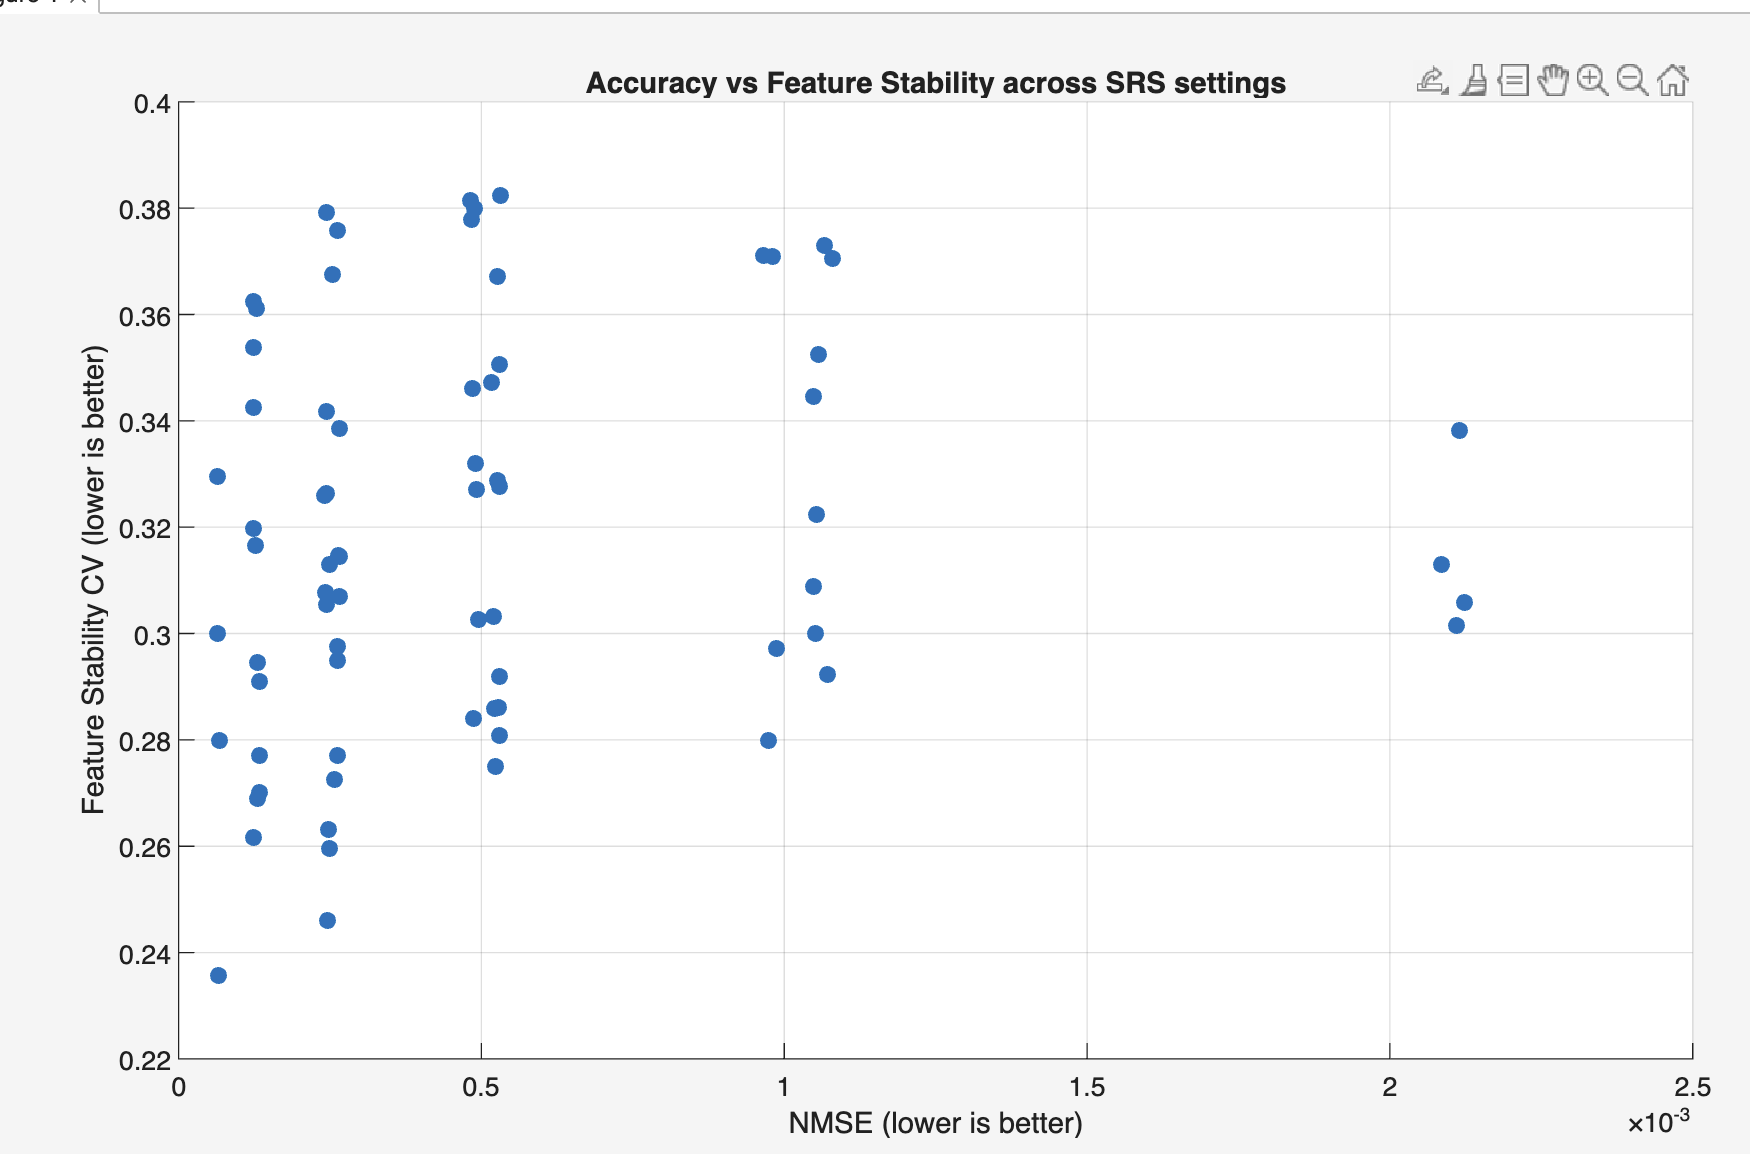
\includegraphics[width=0.8\linewidth]{figures/Scatter Plot.png}
    \caption{Relationship between channel estimation accuracy (NMSE) and sensing feature stability (CV).}
    \label{fig:accuracy_feature_stability}
\end{figure}

\subsection{Performance Metrics}

Two metrics were used to evaluate the performance of the SRS configurations: channel estimation accuracy and sensing feature stability.

\subsubsection{Normalized Mean Squared Error (NMSE)}

Channel estimation accuracy was measured using the Normalized Mean Squared Error (NMSE), defined as

\begin{equation}
\text{NMSE} = \frac{\|H - \hat{H}\|^2}{\|H\|^2}
\end{equation}

where $H$ represents the true channel response and $\hat{H}$ represents the estimated channel response obtained from the received SRS signal. Lower NMSE values indicate more accurate channel estimation.

\subsubsection{Feature Stability (Coefficient of Variation)}

To evaluate the stability of sensing features across repeated simulations, the coefficient of variation (CV) was used:

\begin{equation}
CV = \frac{\sigma}{\mu}
\end{equation}

where $\sigma$ is the standard deviation of the extracted sensing feature and $\mu$ is its mean value across repeated measurements. Lower CV values indicate more stable sensing features.

\section{Discussion}

The results indicate that the performance of SRS-based sensing is influenced not only by signal processing design but also by protocol constraints imposed by the 5G NR stack. Any sensing approach using SRS must therefore operate within timing, bandwidth, scheduling, and power-control limits defined by the standard. The standards analysis and MATLAB simulations complement each other: the standards review defined the feasible SRS configuration space, while the simulations identified which configurations produce stronger sensing performance.

As summarized in Table~\ref{table:srs_results}, the lowest NMSE values were consistently achieved using configurations with four SRS symbols, comb spacing of four, and a bandwidth of 24 resource blocks. Among the evaluated parameters, the number of SRS symbols had the strongest impact on channel estimation accuracy. Configurations using four symbols consistently outperformed those using a single symbol, reducing NMSE from approximately $5 \times 10^{-4}$ to about $6 \times 10^{-5}$. This nearly order-of-magnitude improvement suggests that symbol count is a key parameter when configuring SRS for sensing-oriented applications.

Fig.~\ref{fig:accuracy_feature_stability} further illustrates the relationship between channel estimation accuracy and sensing feature stability across the evaluated configurations. In general, configurations that produced lower NMSE values also yielded more stable sensing features. However, some configurations exhibited a trade-off between estimation accuracy and feature consistency, indicating that optimizing sensing performance requires balancing multiple design parameters.

These observations are consistent with prior wireless sensing research demonstrating the importance of exploiting structured signal information to improve sensing performance. For example, systems such as SpotFi use channel state information from WiFi signals to estimate multipath characteristics and achieve median localization accuracy of approximately 40~cm using commodity hardware \cite{article}. While SpotFi evaluates end-to-end positioning accuracy in WiFi networks, the present study focuses on intermediate sensing metrics—specifically channel estimation accuracy and sensing feature stability—within the constraints of the 5G NR SRS framework. Although the two approaches target different stages of the sensing pipeline, both highlight the value of structured pilot signals and multipath information for improving sensing performance.

Within the evaluated configuration space, SRS settings with moderate bandwidth and comb spacing of four provided strong overall performance, particularly when combined with four SRS symbols. However, these results should be interpreted with caution because the current simulation framework does not include strong time-varying channel effects. This likely explains the relatively small observed influence of SRS periodicity, which may play a more significant role in dynamic environments.

Practical sensing performance may also be affected by higher-layer behavior in real networks. If SRS is configured as aperiodic, sensing measurements occur only when triggered, and MAC-layer scheduling decisions may delay or skip SRS transmissions. Additionally, uplink power control complicates the interpretation of received SRS amplitude because changes in signal strength may reflect transmit-power adjustments rather than environmental variations.

Overall, the results narrow the search toward SRS configurations that are both protocol-compliant and technically promising for sensing. These findings provide a foundation for future experiments involving jammer detection and localization in more realistic network environments.

\section*{Acknowledgments}

This work was conducted as part of the Master of Electrical and Computer Engineering program at Rice University. The authors acknowledge the academic support and institutional resources provided by Rice University, as well as the guidance and feedback from the project advisor throughout the project. The authors also recognize the collaborative contributions of all team members in completing this research. The statements made in this work are solely the responsibility of the authors.


\section{CRediT Author Statement}

\textbf{Sandra Mansour:} Software, Formal analysis, Visualization, Writing--Original draft preparation. \textbf{Samanvitha Balijepalli:} Investigation, Algorithm analysis, Writing--Reviewing and Editing. \textbf{Aniket Jadhav:} Investigation, Methodology, Software. \textbf{Dr. Rahman Doost:} Conceptualization, Supervision, Project administration, Resources, Writing--Reviewing and Editing.

\bibliographystyle{IEEEtran}
\bibliography{references}


\end{document}
